\begin{figure}[H]
    \centering
    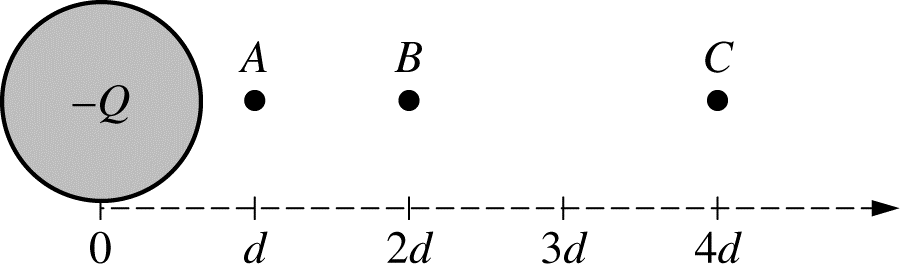
\includegraphics[scale=0.3]{images/img-015-041.png}
\end{figure}

% Multiple Choice Question 34
\begin{questions}\setcounter{question}{33}\question
A particle of charge $+q$ is released from rest at position $B$, which is a distance $2 d$ from the center of a fixed nonconducting sphere that has a charge of $-Q$ distributed uniformly throughout its volume, as shown in the figure above. When the particle reaches position $A$, which is a distance $d$ from the center of the charged sphere, its kinetic energy is $K_{0}$. The same particle is now released from rest at position $C$, which is a distance $4 d$ from the center of the nonconducting sphere. The kinetic energy of the particle when it again reaches position $A$ is

\begin{oneparchoices}
\choice $K_{0}$
\choice $3 K_{0} / 2$
\choice $2 K_{0}$
\choice $5 K_{0} / 2$
\choice $3 K_{0}$
\end{oneparchoices}\end{questions}
